\chapter{Implementation}

Now that we have discussed the design of our system, we will discuss its implementation.
This design will consist of two main parts:

\begin{enumerate}
	\item{Identical Kademlia user nodes which will make up the Kademlia network.
	The code for these nodes will contain implementation for content look-up, publishing and down-voting and will provide 
	a high-level interface for interfacing with the system. }
	\item A user-facing front-end which will have the ability to look-up content, publish content and down-vote content.
\end{enumerate}

We will first discuss general implementation details, then turn our attention to the implementation of these parts.

\section{The Python programming language}

The project was written using the programming language Python. Python is a high-level interpreted programming language with
light syntax and ``duck-typing'', making it ideal for rapid development. Python also has many useful libraries available,
many of which are open-source under permissive licenses. While none of these factors were essential to the development
of the project, the availability of Python libraries helped with the implementation of the system.

\section{Kademlia Implementations}

While there are several available Python implementations of the Kademlia DHT, many are incomplete or badly documented.
We will discuss the available implementations and their relative advantages and disadvantages.

\subsection{Entangled}

Entangled is a working implementation of the Kademlia DHT written in Python. It provides a high-level programming interface and
a graphical interface for interfacing with the Kademlia network with the ability to demonstrate file-sharing graphically.
Entangled also includes an extra ``delete'' RPC which could be easily modified to serve the purpose of the ``down-vote'' RPC
that our system requires. However, Entangled lacks comprehensive documentation and has a complicated API.
Entangled's code-base is complicated and difficult to understand in places. For this reason, it was decided that Entangled
was not suitable to be used for this system.

Entangled is released under the GNU General Public License, v3 (GPLv3).

\subsection{``Kademlia'' Library}

``Kademlia'' is a Kademlia DHT implementation in Python. ``Kademlia'' seems to be well-documented and written,
but as its first release was published after the beginning of this project, it was decided that it would be too unstable of
a platform to base the project on.
However, the library looks promising and it would be possible for it to be used in future projects once the code-base
has become stable.

``Kademlia'' is released under the MIT license.

\subsection{PyDHT}

PyDHT is a pure Kademlia DHT implementation written in Python. PyDHT does not add extra functionality to the DHT, and its code
is simple enough to be understood, despite its lack of documentation. The code-base of PyDHT is small and modular, making
it possible to easily change the implementation in places. PyDHT includes simple code examples demonstrating how to use the
library. As a result, it was decided that PyDHT would be a suitable base to work on for this project.

PyDHT is released under the BSD 2-clause license.

\subsection{Choice of Kademlia implementation}

It was decided that PyDHT would be used as the base of this project due to its stability, simple API and permissive license.
Since PyDHT is licensed under the 2-clause BSD license, we have forked the library and the modified library will be made
available under the same 2-clause BSD license. The modified library will be made available in Appendix 1.

\section{Cryptography}

\subsection{Key Derivation Functions \& MAC}

The implementation of key-derivation functions and MAC used in the project is written using the PyCrypto Python cryptography library ~\cite{pycrypto}.
The code for this implementation is based on PyCrypto code examples released in to the public domain by Brendan Long ~\cite{kdfexample}.
PyCrypto was chosen due to its proven stability and usage as well as it having functional examples of Key-Derivation Functions.

The key-derivation function chosen to be used for this project was PBKDF2. PBKDF2 was written by RSA labs to replace an earlier standard,
PBKDF1, which could only produce keys with length of up to 160 bits ~\cite{kdf}. PBKDF2 is suitable due to it supporting the generation of
larger keys than 160 bits. This ensures that key-sizes can be increased beyond 160 bits in the future if necessary.
PBKDF2 was chosen due to a readily available implementation being included in the PyCrypto library.
Other key-derivation functions that supported large key-sizes would also be suitable for usage in this system.

The MAC algorithm which was chosen to be used for this project was Hash-based Message Authentication Code (HMAC). HMAC was chosen due to a readily
available implementation being provided in the PyCrypto library and due to it being well-known and proven in the field.
Other MAC algorithms would also be suitable in its place.

\subsection{Hashing function}

The hashing function chosen to be used to derive content locations from UUIDs in the system was SHA-1. This could be replaced with any hashing function
that provided a relatively large key-space. SHA-1 was chosen due to an implementation in the Python standard ``hashlib'' library.

\subsection{Cryptographic keys}

Cryptographic keys are necessary to provide encryption and decryption of data stored by nodes on the network. In order to ensure document anonymity,
the encryption scheme used must be strong enough that it would be infeasible for a node on the network to break it in a reasonable amount of time. The user that publishes some data must be able to encrypt that data, and also allow users to decrypt it.

During the design of the system, we considered both symmetric key encryption and asymmetric key (public-private key) encryption.

Asymmetric-key RSA encryption was initially used for encryption and decryption of content. In RSA, a private-key is used for 
decryption and a public-key for encryption ~\cite{rsa}. Since the system requires that the author encrypts a piece of data and readers decrypt it, the private key would have to be given to users to decrypt web-page data. As a result, asymmetric-key
encryption was decided to be unsuitable for the system.

Symmetric-key encryption uses one cryptographic key for both encryption and decryption. This fits the requirements of our design
specification - the content author and content reader can both use the same cryptographic key for encryption and decryption.
This implementation of the system uses Rijndael AES as its implementation of symmetric-key encryption due to its availability
in the PyCrypto library ~\cite{pycrypto}. Rijndael AES was arbitrarily chosen as it has been proven by its industry use, and had no obvious disadvantage compared to the other algorithms.

\section{Code Structure}

The code is split into two major components, as mentioned previously:
\begin{enumerate}
	\item{A Kademlia-based peer-to-peer network. Since the project uses the PyDHT Kademlia implementation library as a base, most of the code is contained in a modified version of PyDHT.
	This part of the code will provide a Python interface to publish, retrieve and down-vote web-pages as well as handling communication with the underlying Kademlia network.}
	\item{The user-facing front-end code. This part of the code will provide a user interface which will allow a user to publish, retrieve and down-vote web-pages
	on the network. This part of the code-base be composed of two parts:
		\begin{enumerate}
		    \item A Python-based program which will relay messages from the user interface to the underlying modified Kademlia network.
			\item A web-browser-based application which provides a user interface to the network. This will be written in HTML and JavaScript, using web-sockets to communicate
			with the Python program which in turn communicated with the Kademlia network.
		\end{enumerate}
	}
\end{enumerate}

We will now continue to discuss the implementation of both of these components.

\subsection{Kademlia-based Peer-to-Peer Network}

This part of the code is heavily based upon PyDHT, which provides a working Kademlia network as a base on which we build the extra features needed by our network.

\subsubsection{Content Publishing  - \texttt{publish(content)}}

Content publishing is done according to the algorithm described in figure \ref{fig:retrievalalgo}, in the Design section of this paper. This is done in the
publish() function of the DHT class in the source file pydht.py. The function generates a random UUID using the standard Python ``uuid'' library, then derives
the content-location using SHA-1 as the hash function. The function then uses the do\_encrypt() function from the key\_derivation module
to encrypt the data, using the UUID, then stores it in the Kademlia network and returns the UUID.

\subsubsection{Content Retrieval - \texttt{retrieve(uuid)}}

Content retrieval is done according to the algorithm described in figure \ref{fig:publishalgo}, in the Design section of this paper. This is done in the
retrieve() function in the DHT class in the source file pydht.py. The retrieve() function takes the given UUID, and uses the hash function to derive the
content-location. The function then retrieves this content from the Kademlia network, and tries to decrypt it using the do\_decrypt() function from the
key\_derivation module, using the UUID. If either the decryption or MAC checking fails, then the function throws an error. Otherwise, the decrypted data
is returned to the user.

\subsubsection{Encryption \& Key Derivation}

The encryption and key-derivation logic of the system is contained in a key\_derivation Python module which was added to PyDHT. The encryption and decryption functions
written in this module are based on code examples released into the public domain ~\cite{kdfexample}.

This module is comprised of the following functions:

\begin{itemize}
	\item {\texttt{make\_key()} \\
	This function takes a UUID and uses a key-derivation function to generate a cryptographic key.
	This key can then be used to as an AES or HMAC key.
	}
	\item {\texttt{make\_hmac()}\\
	This function takes a message and a cryptographic key and uses the key to create a HMAC verification code of
	the message. This HMAC verification code can then be used for message authentication.
	}
	\item {\texttt{encrypt()}\\
	This function takes a message and a cryptographic key and uses the key to encrypt the message using AES.
	}
	\item {\texttt{decrypt()}\\
	This function takes an encrypted message and a cryptographic key and attempts to decrypt the message using the key.
	An error is thrown if this is unsuccessful.
	}
	\item {\texttt{do\_encrypt()}\\
	This is a simple wrapper function that takes a UUID and a message and returns an encrypted message and HMAC verification code. This function uses
	make\_key to generate an AES key and a HMAC key using the UUID, then encrypts the data and generates a HMAC verification code.
	}
	\item {\texttt{do\_decrypt()}\\
	This is a simple wrapper function that takes a UUID and encrypted message and attempts to decrypt and verify it.
	The function generates a HMAC key and an AES key using make\_key, then attempts to decrypt and verify the encrypted data using them.
	If the verification or decryption fails, the function throws an error. Otherwise, decrypted data is returned.
	}

\end{itemize}

\subsubsection{``Down-vote'' Content Censorship Algorithm}

Down-vote handling is done in the logic of the DHT class. The DHT class keeps a record of the TTL and aggregate down-vote count for each of the pieces of
data that it holds. Once per second, the \texttt{tick()} function is called, which adjusts the TTL of items according to their rating. Once an item's TTL
is less than zero, it is deleted from the network. Figure \ref{fig:code-downvote} shows a code listing taken from the tick() function from the
program source, demonstrating the down-vote algorithm's implementation.

\begin{figure}[H]
	\begin{lstlisting}
for (uuid, rating) in self.webpage_ratings.items():
	if rating < 0:
	    downvote_val = math.log(rating, 2)
	    self.ttls[uuid] -= downvote_val
for (uuid, ttl) in self.ttls.items():
    if ttl <= 0:
        print "UUID", uuid, " past TTL - deleting"
        del self.data[uuid]
	\end{lstlisting}
    \caption{Code listing demonstrating how an item is selected for deletion based on its downvote rating.}
    \label{fig:code-downvote}
\end{figure}

\subsection{User-facing front-end}

As mentioned previously, the front-end is made up of of a JavaScript and HTML web-based front-end, and a Python program which
interfaces with the modified Kademlia network. We will now discuss both of these.

\subsubsection{Browser code - \texttt{websocket-client.html}}

The browser code consists of a simple HTML page which provides inputs for users to open pages for a given UUID, to publish pages,
and to down-vote a page that is currently loaded. The page uses JavaScript to draw requested pages to a section of the browser screen,
sending requests to a local Python interface to the Kademlia network using the JSON serialisation format over a web-socket connection.

\subsubsection{Local node - \texttt{websocket-node.py}}

The Python ``local node" provides the web-based front-end an interface to the Kademlia network. The node simply listens on a web-socket connection
and then relays any requests to the underlying Kademlia network.

The web-socket Python code was adapted from an example in the source code of the AutobahnPython project ~\cite{websocket}, which is released
under the Apache license.

\begin{figure}[H]
    \centering
    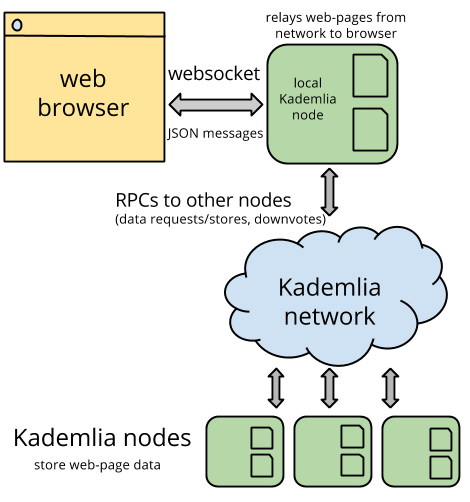
\includegraphics[width=0.6\textwidth]{img/arch-frontend.png}
    \caption{A diagram showing the system architecture, including the user-visible front-end.}
    \label{fig:arch-frontend}
\end{figure}

\subsection{Demonstration shell \& Python scripts}

In order to demonstrate the running of the program, a shell script was included with the project in the
file \texttt{src/demo.sh}.
The script does the following:
\begin{enumerate}
    \item {Creates an initial node that starts the Kademlia-based network}
    \item {Opens ten instances of the xterm terminal emulator which start other nodes
        which then join the network. Messages received by these nodes from the network
        are printed in real-time.}
    \item {Opens a `front-end' node, which listens on a web-socket connection for the front-end.
        This node also joins the Kademlia-based network as a normal user.}
    \item {Opens the web front-end in the Firefox browser. A user can then store and retrieve
        web-pages in the network, and down-vote them.}
\end{enumerate}

This shell script is designed to run on GNU/Linux and has not been tested in other environments.

As well as this shell script, two files \texttt{create\_network.py} and \texttt{join\_network.py}
are provided to create a network and join nodes to it.
